\section{TD 21}



\subsection{Rappels}


\paragraph{Trigonométrie}

\begin{align*}
	sin(x)= \frac{e^{ix}-e^{-ix}}{2i} &&&&& cos(x)=\frac{e^{ix}+e^{-ix}}{2} \\
	e^{ix}= \cos x+i\sin x &&&&& \cos^2 x+\sin^2 x=1 \\
	cos(x)=cos(-x) &&&&& sin(x)=-sin(-x)
\end{align*}


\paragraph{Les énergies}

Dans le cadre de la résolution de l'équation de schrodinger avec un hamiltonien réduit au terme de translation on peut rencotrer 2 cas:
\begin{itemize}

	\item État non lié 

	\begin{align*}
		H|\phi \rangle = E |\phi \rangle &&&&& E>0 \\
		\Rightarrow k=\sqrt{\frac{2mE}{\hbar^2}} &&&&& \phi (x) =Ae^{ikx}+Be^{-ikx}
	\end{align*}

	\item État lié

	\begin{align*}
		H|\phi \rangle = E |\phi \rangle &&&&& E<0 \\
		\Rightarrow k=\sqrt{\frac{-2mE}{\hbar^2}} &&&&& \phi (x) =Ae^{kx}+Be^{-kx}
	\end{align*}

\end{itemize}


\subsection{Notions importantes}


\paragraph{Densité d'états et nombre moyen d'occupation}

La densité d'états $g(k)$ ou $g(E)$ représente la quantité $\frac{dN}{dE}$ à ne pas confondre avec le nombre moyen d'occupation $\bar{n}$ qui lui représente le nombre moyen de particules dans chaque un des états contenus dans $g(E)dE$.


\paragraph{La masse effective}

On parle de masse effective lorsqu'on réalise un développement de Taylor autour d'un extremum de l'énergie. En fonction des 2 cas présentés plus haut ou trouve une énergie en $\alpha x^2$ ou en 
$-\alpha x^2$. La masse effective est en fait la masse fictive qui apparait dans le développement. On observe que dans les cas antérieurs il y a simplement un changement de signe.


\paragraph{La théorie des barres}

On introduit ici une théorie qui sera importante dans ce TD ainsi que dans le suivant. On sait que le spectre énergétique d'un atome est discret. Un solide est un ensemble d'atomes, de par le principe de d'exclusion les électrons de l'atome ne vont pas pourvoir se placer tous sur les mêmes énergies, ils vont interagir et créer des variations autour des énergies discrètes en laissant apparaitre des bandes d'énergies possibles et interdites (voir figure ci-dessous).

\begin{figure}[H]
	\begin{center}
		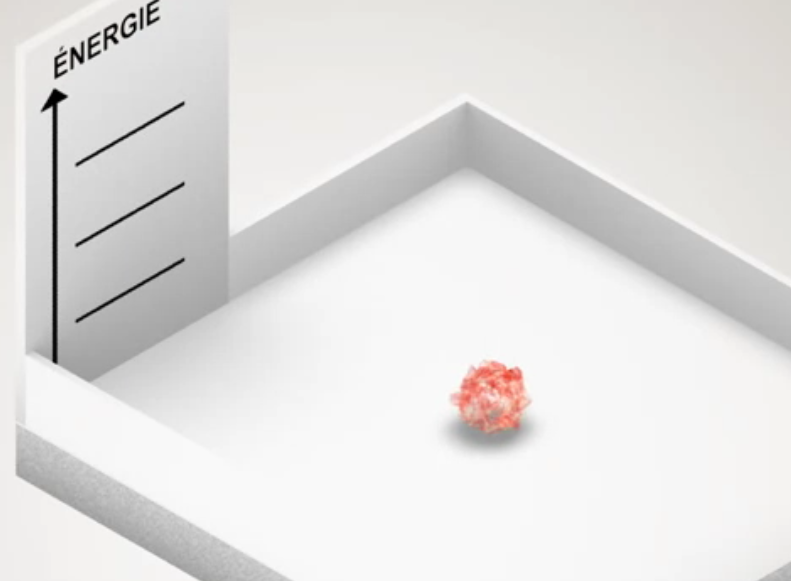
\includegraphics[scale=0.2]{./img/IM5}
		\caption{Un atome et son spectre énergétique quantifié}
	\end{center}
\end{figure}

\begin{figure}[H]
	\begin{center}
		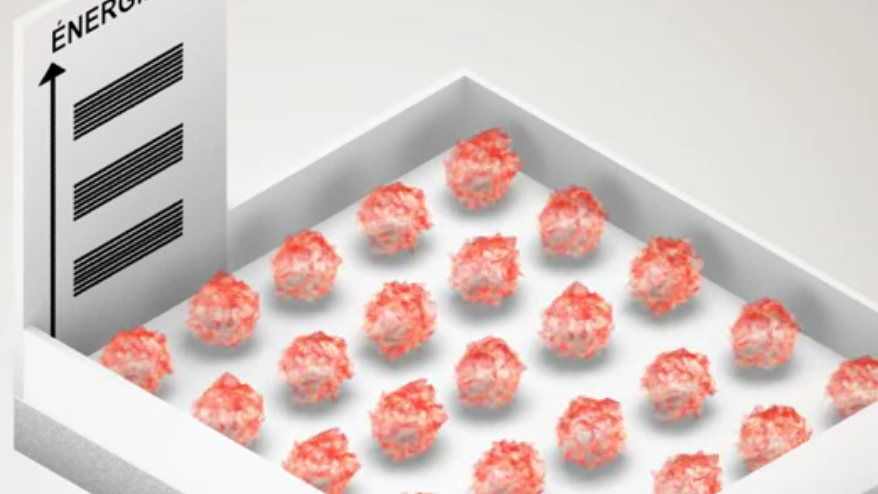
\includegraphics[scale=0.2]{./img/IM6}
		\caption{Plusieurs atomes et la modification du spectre énergétique}
	\end{center}
\end{figure}